\documentclass[11pt]{article}
\usepackage[margin=1in]{geometry}
\usepackage{parskip}
\usepackage{listings}
\usepackage{xcolor}
\usepackage{titlesec}
\usepackage{hyperref}
\usepackage{amsmath}
\usepackage{amssymb}
\usepackage{tikz}
\usepackage{array}
\usepackage{booktabs}
\usepackage{float}
\usetikzlibrary{matrix, positioning}

\hypersetup{colorlinks=true, linkcolor=black, urlcolor=blue}

\titleformat{\section}{\large\bfseries}{}{0em}{}[\titlerule]
\titleformat{\subsection}{\normalsize\bfseries}{}{0em}{}

\lstset{
	language=Python,
	basicstyle=\ttfamily\footnotesize,
	keywordstyle=\color{blue}\bfseries,
	commentstyle=\color{gray}\itshape,
	stringstyle=\color{teal},
	breaklines=true,
	frame=single,
	rulecolor=\color{black!30},
	backgroundcolor=\color{black!3},
	numbers=left,
	numberstyle=\tiny\color{gray},
	xleftmargin=1.5em,
	framexleftmargin=1.5em
}

\title{
	\LARGE\textbf{15-Puzzle Solver} \\[0.4em]
	\large IDA* Search with Manhattan Distance and Linear Conflict
}
\author{Evan Washington}
\date{}

\begin{document}
	
	\maketitle
	
	% ── Section 1 ────────────────────────────────────────────────────────────────
	\section{Introduction}
	
	The 15-puzzle is a combinatorial search problem consisting of a $4 \times 4$ 
	grid containing tiles numbered $1$--$15$ and one blank space. A move consists 
	of sliding any tile orthogonally adjacent to the blank into the blank's 
	position. The goal is to reach the canonical ordering:
	
	\[
	\begin{pmatrix}
		1 & 2 & 3 & 4 \\
		5 & 6 & 7 & 8 \\
		9 & 10 & 11 & 12 \\
		13 & 14 & 15 & \square
	\end{pmatrix}
	\]
	
	The state space has size $\frac{16!}{2} = 10{,}461{,}394{,}944{,}000$ reachable 
	configurations, making uninformed search intractable. This project implements 
	an optimal solver using Iterative Deepening A* (IDA*) guided by a composite 
	admissible heuristic. The program accepts random or user-defined boards, 
	validates solvability, solves optimally under a 3-minute timeout, and logs 
	full step-by-step solutions to disk.
	
	% ── Section 2 ────────────────────────────────────────────────────────────────
	\section{State Representation and Solvability}
	
	\subsection{Representation}
	
	Each board state is encoded as a 16-element Python \texttt{tuple}, where index 
	$i$ holds the tile at row $\lfloor i/4 \rfloor$, column $i \bmod 4$, and 
	$0$ denotes the blank. Tuples are chosen for immutability and hashability, 
	enabling $O(1)$ membership tests in the visited-state set during search.
	
	\subsection{Solvability}
	
	Define an \textit{inversion} as any pair $(i, j)$ with $i < j$, $s_i \neq 0$, 
	$s_j \neq 0$, and $s_i > s_j$ in the flattened board $s$; letting $N$ denote 
	the total inversion count and $r$ the row of the blank counted from the bottom 
	(1-indexed), a configuration is solvable if and only if 
	$(r \text{ even} \;\wedge\; N \text{ odd}) \;\vee\; (r \text{ odd} \;\wedge\; N \text{ even})$. 
	If a randomly generated board fails this condition, solvability is restored by 
	swapping any two non-blank tiles, which changes $N$ by an odd number without 
	displacing the blank, flipping the parity of $N$ and satisfying the criterion.
	
	% ── Section 3 ────────────────────────────────────────────────────────────────
	\section{Heuristic Function}
	
	\subsection{Manhattan Distance}
	
	A heuristic function estimates the cost remaining from a given state to the 
	goal, allowing the search to prioritise more promising paths. For this to 
	guarantee an optimal solution, the heuristic must be \textit{admissible}, 
	meaning it never overestimates the true cost. Manhattan distance is one such 
	heuristic: it measures the minimum number of moves each tile would require to 
	reach its goal position if it could slide freely without interference from 
	other tiles. Since tiles do block each other in practice, this is always an 
	underestimate, satisfying admissibility.
	
	For tile $v$ at position $i$, its goal position is index $v - 1$. The 
	Manhattan distance contribution of tile $v$ is:
	
	\[
	d(v, i) = \left|\left\lfloor\frac{i}{4}\right\rfloor - \left\lfloor\frac{v-1}{4}\right\rfloor\right|
	+ \left|(i \bmod 4) - ((v-1) \bmod 4)\right|
	\]
	
	The total Manhattan heuristic is:
	\[
	h_{\text{MD}}(s) = \sum_{\substack{i=0 \\ s_i \neq 0}}^{15} d(s_i,\, i)
	\]
	
	\subsection{Linear Conflict}
	
	Manhattan distance treats each tile independently, but in practice tiles 
	frequently block each other even when both are in their correct row or column. 
	Linear conflict captures this: if two tiles both belong in the same row but 
	are currently in the wrong order relative to each other, they must pass each 
	other, requiring at least one tile to vacate the row and re-enter. This adds a 
	minimum of 2 moves per conflicting pair that Manhattan distance alone does not 
	account for. Two tiles $t_a$, $t_b$ are in \textit{linear conflict} in a row 
	$r$ if both have their goal positions in row $r$, and $t_a$ is to the left of 
	$t_b$ currently but $t_a$'s goal is to the right of $t_b$'s goal. The same 
	applies column-wise. The combined heuristic is:
	
	\[
	h(s) = h_{\text{MD}}(s) + 2 \cdot \bigl(C_{\text{row}}(s) + C_{\text{col}}(s)\bigr)
	\]
	
	where $C_{\text{row}}$, $C_{\text{col}}$ count conflicting pairs per row and 
	column respectively. This heuristic remains admissible and dominates 
	$h_{\text{MD}}$ alone, substantially reducing the number of nodes expanded 
	during search.
	
	\begin{figure}[H]
		\centering
		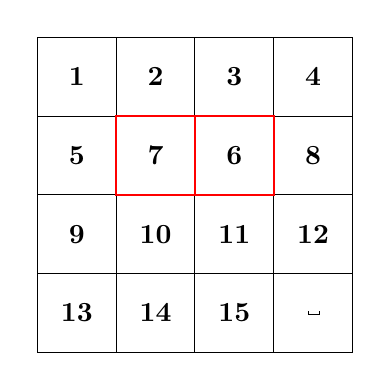
\begin{tikzpicture}
			\matrix (m) [matrix of nodes,
			nodes={draw, minimum size=1cm, anchor=center, font=\bfseries},
			column sep=-\pgflinewidth,
			row sep=-\pgflinewidth]{
				1 & 2 & 3 & 4 \\
				5 & 7 & 6 & 8 \\
				9 & 10 & 11 & 12 \\
				13 & 14 & 15 & \textvisiblespace \\
			};
			\node[draw=red, thick, minimum size=1cm, anchor=center] at (m-2-2) {};
			\node[draw=red, thick, minimum size=1cm, anchor=center] at (m-2-3) {};
		\end{tikzpicture}
		\caption{Tiles 6 and 7 are in linear conflict: both belong in row 2 but are 
			reversed. Resolution requires at least 2 extra moves beyond Manhattan distance.}
	\end{figure}
	
	% ── Section 4 ────────────────────────────────────────────────────────────────
	\section{IDA* Search Algorithm}
	
	IDA* (Iterative Deepening A*) is a memory-efficient variant of the classical 
	A* search algorithm. Where A* maintains a priority queue of all discovered 
	states in memory, which grows exponentially with search depth, IDA* instead 
	performs a series of depth-first searches each bounded by a cost threshold. 
	This reduces memory usage from $O(b^d)$ to $O(d)$, where $b$ is the branching 
	factor and $d$ is the solution depth, at the cost of re-expanding shallow nodes 
	on each iteration. For the 15-puzzle this trade-off is highly favourable, since 
	solution depths can reach 80 moves and storing all frontier states at that 
	depth would be infeasible.
	
	The threshold $\lambda$ is initially set to $h(s_0)$. At each node the 
	$f$-value is computed:
	
	\[
	f(n) = g(n) + h(n)
	\]
	
	where $g(n)$ is the path cost from the root. If $f(n) > \lambda$, the branch 
	is pruned and $f(n)$ is returned as a candidate for the next threshold. 
	Each iteration raises $\lambda$ to the minimum pruned $f$-value until a 
	solution is found:
	
	\[
	\lambda_{k+1} = \min\{f(n) : f(n) > \lambda_k,\; n \text{ pruned in iteration } k\}
	\]
	
	\begin{lstlisting}[caption={Core IDA* search loop}]
		def search(path, g, threshold):
		state = path[-1]
		f = g + heuristic(state)
		if f > threshold:
		return f                   # prune; f is next threshold candidate
		if state == GOAL_STATE:
		return "FOUND"
		minimum = float("inf")
		path_set = set(path)
		for nb in get_neighbors(state):
		if nb not in path_set:
		path.append(nb)
		result = search(path, g + 1, threshold)
		if result == "FOUND":
		return "FOUND"
		if result < minimum:
		minimum = result
		path.pop()
		return minimum
	\end{lstlisting}
	
	A daemon thread enforces a 180-second wall-clock timeout via a shared flag, 
	allowing clean early termination if the puzzle proves too complex to solve 
	within the time limit.
	
	% ── Section 5 ────────────────────────────────────────────────────────────────
	\section{Testing and Validation}
	
	Eight assertion-based unit tests run automatically before the program starts, 
	covering all core components:
	
	\begin{center}
		\begin{tabular}{clc}
			\toprule
			\textbf{\#} & \textbf{Test} & \textbf{Expected} \\
			\midrule
			1 & \texttt{manhattan(GOAL\_STATE)} & $0$ \\
			2 & Manhattan of one-off board & $1$ \\
			3 & \texttt{is\_solvable(GOAL\_STATE)} & \texttt{True} \\
			4 & Known unsolvable board & \texttt{False} \\
			5 & Neighbors of corner blank & $2$ \\
			6 & Solve already-solved board & path len $1$, explored $= 0$ \\
			7 & Solve one-move board & path len $2$ \\
			8 & \texttt{results.txt} written correctly & timestamp present \\
			\bottomrule
		\end{tabular}
	\end{center}
	
	Any failure halts execution before user interaction begins, ensuring the solver 
	is never invoked in a broken state.
	
	% ── Section 6 ────────────────────────────────────────────────────────────────
	\section{Usage}
	
	
	The program prompts for a random or custom board. Custom input is 16 
	space-separated integers $0$--$15$, each used exactly once, where \texttt{0} 
	is the blank. On completion, the full move-by-move solution is printed to 
	stdout and appended to \texttt{results.txt} alongside metadata (timestamp, 
	move count, states explored, timeout status).
	
	% ── Section 7 ────────────────────────────────────────────────────────────────
	\section{Limitations and Future Work}
	
	Worst-case 15-puzzle instances require up to 80 moves. Although IDA* with 
	linear conflict solves most boards efficiently, deeply scrambled configurations 
	may exceed the timeout after exploring $10^8$+ states. If I decide to revise 
	the project, I would likely do the following. First, implement disjoint pattern 
	databases, which precompute exact move costs for subsets of tiles, this would 
	yield almost perfect lower bounds and would largley reduce total states explorede. Second, replace the recursive implementation with an explicit stack, 
	eliminating the \texttt{sys.setrecursionlimit} dependency entirely. Porting to C++ 
	alongside pattern databases would produce multiplicative gains, C++ reduces 
	the cost of each state evaluation by roughly one to two orders of magnitude, 
	while pattern databases reduce the number of states needing evaluation by a 
	similar factor.
	
\end{document}